\section{Free substitution}\index{variable}\index{substitution}

It is a general reality that attention to domains is an af\-ter\-thought to an
algebra problem, not a forgoing assumption.  In fact if we explore inputs
outside the domain we might discover they are not so bad.  Many of them would
simply lead to complex numbers, and we might arrange for that eventuality.  
What we really have is an understanding of functions as a process to operate 
on data.  Later  we add aspects such as domains and codomains to study them in restricted ways.

So what is a function if we do not have domains and codomains with which to start?

Let us take seriously the idea of simple substitution: replacing $x$ for something else.
Start with something familiar like substituting $4$ for $x$, but to make 
it sporting use Roman numerals.
\[
    f(IV) = \frac{\sqrt{e^{IV}-1}}{IV^2-IV-6}.
\]
This is hideous but at the same time it remains appropriate, we can interpret 
$f$ as applying to $4$ however we choose to represent it.  The same happens with 
the concept of the variable $x$, we can rename it.
\[
    f(t) = \frac{\sqrt{e^{t}-1}}{t^2-t-6}.
\]
The way we know how is wrapped up in the fact that we know 
in principle how to replace $x$ by any symbol, say $x\leftrightarrows \clubsuit$
\[
    f(\clubsuit) = \frac{\sqrt{e^{\clubsuit}-1}}{\clubsuit^2-\clubsuit-6}.
\]
If we need to make sense of expressions like these we might call $\clubsuit$ 
a ``place holder'' for some yet undeclared explanation.  Yet on the otherhand 
I think it best to think of this more similar to  $f(-1)$, which, if used 
would lead to the temporary absurdity of a negative inside a square-root.
It would be unknown perhaps but not disqualifying.

This type of substitution is completely sound.  To make this clear 
we again have simplify the reading of a math formula by searilizing 
the symbols as we did in Section~\ref{sec:cfg}.
In this way everything we write can be discussed as a string $M_1 M_2\cdots M_{\ell}$
of smaller strings $M_i$, even if in reality the layout is more interesting.
This decomposition into smaller strings is not generally unique.  

\begin{remark}{Free choices}
    There are no agreed to conventions that say to read a fraction top-to-bottom
    instead of bottom-to-top, or to read a product of monomial left-to-right
    verses right-to-left. And yet we get the same answers.  Why?\\

    For all the efforts on orders of operations and conventions, there is simply 
    too much variability in how we breakup formulas into strings to ever judge this 
    as unique.  So something else is at play to make all these choices immaterial.
    Notice if a function is truly just the output for every input then this problem 
    does not exist---there are no robbers just their crime scene.
\end{remark}

With this notion of string, let us begin with the general case where everything 
can be replaced.  This means the atoms of the decomposition are restricted to an
alphabet we call ``variables''. That is all it means to be a variable:
\begin{center}
    \textbf{you are a
variable if you are in the alphabet of variables. }
\end{center}

\begin{definition}[Pure substitution]
    Given strings $M$ and $N$, and a variable $x$, to replace $x$ in $M$ by $N$ ,
    denoted here as $M[x\leftrightarrows N]$ by follow these rules.
    \begin{description}
        \item[Free.match] $x[x\leftrightarrows N]\defeq N$.
        \item[Free.other] $M[x\leftrightarrows N]\defeq M$ if $M$ is in the variables alphabet (and 
        because we already will have intercepted the case $M=x$ in the above case we know $M\neq x$).
        
        \item[Free.recurse] $(LM)[x\leftrightarrows N]\defeq L[x\leftrightarrows N]M[x\leftrightarrows N]$
    \end{description}
\end{definition}

A word on notation.  Some authors us $M[N/x]$ or $[N/x]M$ or $M[x/N]$ in place
of $M[x\leftrightarrows N]$.  That notation runs into confusion in algebra
which has other intentions for `/'. 

\begin{remark}{Replace variables don't assign them}
    There is a widely used abbreviation $x\defeq 2$ used 
    in place of $x[x\leftrightarrows 2]$ popular especially to programs.  
    It is common to encounter arguments shaped like the following.  Given:
    \begin{align*}
        M & \defeq x+3 & N & \defeq 2x
    \end{align*}
    ``Assign $x \defeq 2$ to find...''
    \begin{align*}
        M  & = 2+3 =5 & N & = 2\cdot 2 =4
    \end{align*}
    Strictly speaking, $x$ is in the variable alphabet and $2$ in the constant 
    alphabet so no amount of ``assignment'' can turn one into the other.
    The more accurate description is the following:
    \begin{align*}
        % M & \defeq x+3 & N &\defeq 2x\\
        M[x\leftrightarrows 2] & = 2+3=5 & N[x\leftrightarrows 2] & = 2\cdot 2=4.
    \end{align*}
    Confusing replacement with assignment leads eventually to confused 
    results.  For example, if later we reassign $x\defeq 7$ then $M=10$ not 5.
    To unwind this requires that we sequence all uses of $M$ and think of $M$ 
    ``at time/step 1, 2, ...''.  Retaining the substitution notation is 
    on the other hand always accurate.
\end{remark}



% This type of substitution got us into trouble, after all $(K_c(x)=x)[c\leftrightarrows x]$
% would become $x$.



% It will shock no one that given a formula
% \[
%     f(x) = \frac{x}{\sqrt{x^{2}-\frac{5}{3}x}}
% \]
% it is possible to replace $x$ by any symbol I like.  
% Here I swapped $x\leftrightarrows 2$:
% \[
%     f(2) = \frac{2}{\sqrt{2^2-\frac{5}{3}2}}=\frac{2\sqrt{3}}{\sqrt{2}}.
% \]
% To be cute I next used the Roman Numeral $x\leftrightarrows III$
% \[
%     f(III) = \frac{III}{\sqrt{III^2-\frac{5}{3}III}} = \frac{III}{II}.
% \]
% While it is unusual to work with Roman numerals this was in fact 
% valid.  To give it meaning we had to consult some interpretation 
% of Roman numerals as numbers and calculate in that notation. 
% As that worked what about $x\leftrightarrows \clubsuit$:
% \[
%     f(\clubsuit) = \frac{\clubsuit}{\sqrt{\clubsuit^2-\frac{5}{3}\clubsuit}}.
% \]
% At this point we might see this as a step too far.  Perhaps we might observe 
% that $\clubsuit$ is not in the domain.

% To call this ``evaluating $f$'' goes too far.  We truly are erasing 
% one symbol and drawing in another.  To emphasize this, suppose 
% we had not been given ``$f(x)=...$'' but instead this:
% \begin{align*}
%     f(x) 
\includegraphics[width=0.5cm]{sheep.jpg} x\sqrt{x^2-x}
%     \qquad 
%     f(\clubsuit) 
\includegraphics[width=0.5cm]{sheep.jpg}\clubsuit \sqrt{\clubsuit^2-\clubsuit}
% \end{align*}
% The substitution worked just as well and our only concern now is will the sheep eat 
%  the clovers $\clubsuit$.  

% This silly illustration points out that $f(x)=...$ 
% is tempting us to put too many assumptions on what the symbols mean.
% For example you might have thought there was an implied domain of decimal numbers.
% After all square-roots often turn up for decimals.  And yet that cannot be 
% enough motivation because all of us will, if we are honest most of use will on occasion 
% attempt to evaluates such a function at a number that wont make sense long term.


% , and if treated 
% just as symbols our minds may no longer lead us to a misunderstanding.  The locations
% of a fixed symbol are what matter, not the symbol itself.

% Given that location matter, notice that formulas use an array of locations:
% left-right $LM$, e.g.\ $(x+2)(x+3)$; up-down $\overset{L}{M}$, e.g.\ $\frac{x+2}{x+3}$
% on the diagonals $L^M$, e.g.$(x+2)^{(x+3)}$, in three dimensions, e.g. a tensor product $u\otimes v\otimes w$
%     \begin{center}
%         \includegraphics[width=2in,page=26]{Tensor-Product-Def-3D.pdf}
%     \end{center}
% The trouble is that when exploring substitution we want to give a step-by-step 
% description, not including nuances of locations.  So, actual location not-withstanding,
% when we decompose a formula we shall narrow 
% our notation to inline, so $N=LM$ and think of the result as a ``string'' reading 
% left-to-right.

Often in our applications it makes sense to leave some symbols fixed.
For example $0,1,2,3,\ldots$ or the number $\pi$ might not vary in an application.
When this is the case we make a separate alphabet of constants and change substitution 
rules around that alphabet.
\begin{definition}[Applied substitution]
    Given strings $M$ and $N$ with variables or constants, 
    and a variable $x$, to replace $x$ in $M$ by $N$ 
    follow the rules of pure substitution but add a  base case:
    \begin{description}
        \item[Constant] $c[x\leftrightarrows N]\defeq c$ when $c$ is a constants alphabet. 
    \end{description}
\end{definition}

Towards our earlier point in Chapter~\ref{chp:what-is-algebra}, pure algebra has no constants.
